
\section{Related Works}
\label{sec:literature}

\subsection{Systematic Literature Review process}

This SLR aims at tackling RQ1. More precisely, the following research questions will be answered:

\begin{itemize}
    \item [RQ1.1] What is the current state-of-the-Art for DAG task scheduling with precedence constraints ?
    \item [RQ1.2] How has LET been used in scheduling event-chains ?
    \item [RQ1.3] What machine learning techniques have been used for scheduling tasks on real-time systems ?
\end{itemize}
It will also be shown how the literature doesn't provide 
a complete answer to RQ2, hence the contributions of this paper.\\

From these research questions, several concepts have been isolated,
namely, time-triggered tasks, the nature of the system (real-time multicore system),
the scheduling of tasks, DAG tasks, and machine learning.
The recording of the search results were done using the BibTeX LateX plugin
combine with the google scholar "cite" feature.

Searching was conducted using the IEEE and ACM databases.
According to the concepts identified above, 
the keyword chain used for searching was 
"("real-time" OR "real time") AND 
"system" AND ("time-triggered" OR "time triggered" OR "DAG" OR "Directed Acyclic Graph" OR "LET" OR "Logical Execution Time" OR "event chain" OR "event-chain") 
AND "task" 
AND ("scheduling" OR "scheduler" OR "schedule") 
AND ("multi-processors" OR "multi-cores" OR "multi processors" OR 
"multi cores" OR "multi-processor" OR "multi processor" OR 
"multi-core" OR "multi core")".

The search produced 3,549 results on the IEEE database
which was reduced tp 1,171 papers when considering only 
articles published in the past 5 years.

Then the following exclusion criterias were used to filter out 
the rest of the articles, bringing the number of papers down to 19
(see Figure \ref{fig:slr_process}).

\begin{itemize}{}{}
    \item [EC1] Not focusing on homogeneous multicores and hard RTS
    \begin{list}{}{}
        \item "Heterogeneous" not in the title nor the abstract.
        \item "mixed critical*" not in the title nor the abstract
    \end{list}
    
    \item [EC2] Not focusing on scheduling
    \begin{list}{}{}        
        \item "scheduling" or "scheduler" or "schedule" in the title 
        \item "energy" not in the title
        \item Focus on conference and journal papers
    \end{list}

    \item [EC3] Not focusing on real-time systems, not proposing a scheduling algorithm, not using DAG, LET or event-chain tasks.
\end{itemize}

\begin{figure}[htbp]
    \centering
    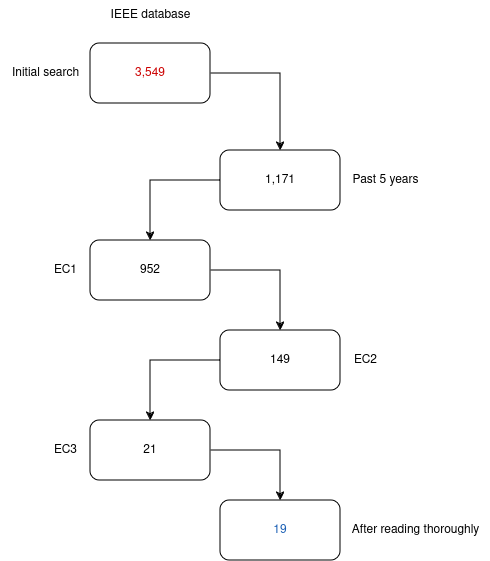
\includegraphics[width=\linewidth]{images/slr_process.drawio.png}
    \caption{SLR process diagram. EC stands for Exclusion Criteria,
    which are listed above.}
    \label{fig:slr_process}
\end{figure}


\subsection{Findings of the Literature Review}
 
In \cite{guan2021DAGfluid}, authors 
use fluid scheduling to schedule multiple DAG tasks
on a multicore system. 
Fluid scheduling has been used in previous work for independent
time-triggered task scheduling\cite{baruah1993PFair}\cite{cho2006LLREF} 
but very few consider DAG tasks. Fluid-scheduling is known for producing optimal scheduling algorithms.
Their method decomposes a DAG task into several sequential segments
in which the subtasks will execute according to the fluid scheduling 
model. Although their algorithm significantly outperforms
existing algorithms, the main limitation that is common to all fluid-based
scheduling algorithm is the runtime overhead induced by the fluid-scheduling model.
Although authors in \cite{guan2021DAGfluid} briefly explain how 
to transform their scheduling algorithm to a non-fluid one for practical implementation,
they do not evaluate the overhead caused by the frequent task migrations
and preemptions. Also, their algorithm only considers DAG task with implicit deadlines
(D = T) which makes the response-time analysis simpler but to the cost
of generalizability.

As a follow up, authors in \cite{GuanFluidDag2022} 
extend the fluid scheduling algorithm in \cite{guan2021DAGfluid}
to constrained and arbitrary deadline tasks,
especially focusing on DAG tasks with a deadline greater than their period.
Their main contributions are their new scheduling algorithm that 
performs better than existing methods in terms of acceptance ratio,
and producing the first theoretical capacity bound for DAG tasks
with deadlines greater than their periods.
However, the authors still don't provide any evaluation 
on the amount of runtime overhead their scheduling algorithm implementation
produces which generally lowers the actual acceptance ratio
of the algorithm. 

Instead of considering fluid-scheduling,
a popular scheduling method is federated scheduling.
Federated scheduling is based on the idea
of assigning heavy tasks ($U > 1$) to multiple cores
for the whole duration of the tasks' executions,
and assigning light tasks ($U \le 1$) to execute on
cores that have not been assigned a heavy task.
Although it is popular, it suffers from a resource wasting problem,
especially when the difference between the critical path's length 
and the deadline is small,
which many papers aim at solving
\cite{Guan2023FederatedNew}
\cite{jiangUtilTensityBound}
\cite{JiangVirtuallyFederatedSched2021}
\cite{Jiang2023SchedVirtualProcs}
\cite{Kobayashi2023FedBundledDagsched}
\cite{He2023DegreeOfParallelism}.

\cite{jiangUtilTensityBound}, for instance, 
consider federated scheduling and GEDF
and introduces a better metric called the util-tensity bound
that extends the concept of capacity bound
to have a better schedulability test.
Based on this newly derived bound, the authors 
propose an extension to the classic federated algorithm,
with very low tensity tasks being scheduled with GEDF, 
tasks with high-utilization and relatively high tensities are scheduled
using the classic federated scheduling and low utilization
tasks with relatively high tensities are scheduled using partitioned-EDF.
Their algorithm, based on their newly derived bound, effectively improves
the system schedulability of DAG tasks and reduces the resource wasting 
problem of federated scheduling. The main limitation
of this paper is that they only consider GEDF 
for their util-tensity bound and also only consider implicit deadline DAG tasks.

This problem of resource wasting in federated scheduling
is also tackled in \cite{Kobayashi2023FedBundledDagsched}
where the authors propose a federated and bundled-based scheduling
algorithm which enhances the schedulability of DAG tasks
compared to existing federated scheduling algorithms.
Their method consists of using federated scheduling for
tasks with high critical path to deadline ratio and bundled
scheduling for tasks with low critical path to deadline ratio.
Unfortunately, this paper only looks at 3 DAG tasks to evaluate
their algorithm which is a really small amount and is not 
representative of the different DAG tasks that can exist.

Authors in \cite{JiangVirtuallyFederatedSched2021}
take another approach by proposing a virtually-federated 
scheduling algorithm that leverages the advantages
of federated scheduling while improving the acceptance 
ratio for DAG tasks, outperforming existing algorithms.
Their approach consists of adding a virtual layer
of processors, on top of physical processors,
and apply their federated-based scheduling algorithm on those virtual processors,
thus enabling tasks to share a physical processor
even though they are assigned to different virtual processors.
The main drawback in \cite{JiangVirtuallyFederatedSched2021}
is that they only consider the heavy tasks (i.e., $U > 1$)
and do not take the light tasks into account.

To fix this limitation, \cite{Jiang2023SchedVirtualProcs}
extend their previous work\cite{JiangVirtuallyFederatedSched2021}
so that it considers both heavy and light tasks.
The resulting virtually federated scheduling algorithm
clearly outperforms any other federated-based scheduling algorithms
in terms of acceptance ratio.
However, they still only consider implicit or constrained deadline tasks
and they don't provide any evaluation of the run time overhead 
their algorithm might induce.


\cite{Guan2023FederatedNew} 
consider arbitrary deadline tasks and especially
DAG tasks that have a deadline that is greater than their period.
They introduce a new federated scheduling algorithm 
that takes those type of tasks into account 
and compare it to existing global or federated scheduling approaches
for arbitrary deadline tasks, significantly outperforming
most of them in terms of acceptance ratio.
Their approach consists of using this new proposed aglgorithm 
for heavy tasks that have a deadline bigger than their period,
then using classic federated scheduling for the heavy tasks with a 
constrained deadline, and finally using EDF-FF for the light tasks.
Although the fluid-based method in \cite{GuanFluidDag2022}
outperforms this new federated scheduling algorithm,
the impracticality of fluid-based algorithm makes this algorithm
the current best, in terms of acceptance ratio, for dealing with arbitrary
deadlines. The main limitation of this work 
is that it doesn't tackle the resource wasting problem 
that classical federated scheduling, or their new algorithm, has or can potentially have, but only
focuses on providing an algorithm for arbitrary deadline tasks.

For constrained deadline DAG tasks, 
\cite{He2023DegreeOfParallelism} propose a federated-based
scheduling algorithm that outperforms on average by more than 18\%
previous SOTA\cite{Jiang2023SchedVirtualProcs} in terms of acceptance
ratio, making this work the current SOTA for constrained deadline multi-DAG scheduling.
Their approach uses the notion of degree of parallelism, which they 
define rigorously, to improve the classic federated scheduling way of 
choosing the number of cores to assign each heavy tasks.
They also propose a new response-time bound for constrained deadline DAG tasks
based on this defined notion.
Although their method clearly stands out,
they don't consider intra-task scheduling at all 
when their motivation came from the notion 
of degree of parallelism being used
but wrongly defined in previous intra-task scheduling work\cite{Zhao2022DAGsched}\cite{zhao2020DAGsched}.\\

Federated scheduling isn't the only method used,
\cite{JiangDecompoSchedParallelTask},
for instance, propose a decomposition-based 
approach to schedule multi-DAG tasks as well as 
a metric for testing the schedulability of tasks.
Their decomposition strategy proves to be the most efficient 
, according to the defined metric, and the scheduling algorithm
derived from it shows promising results in terms of
acceptance ratio.
Their decomposition strategy basically works by first 
definin execution segments and then then assigning subtasks 
to those segments using the laxity\footnote{Laxity is the gap between the total execution time of a task (potentially comprising the I/O delays) and its deadline.} of those subtasks so that 
no segments are overloaded with workload.
The main limitation of this work is that 
they only look at GEDF variants for priority assignment 
and do not evaluate their decomposition method
using other scheduling heuristics for multi-DAGs.
Most of the articles presented up to now 
tackle inter-task scheduling, not considering
the intra-task execution schedule.

Indeed, intra-task scheduling\cite{He2019DagIntra}\cite{Xiao2019}
\cite{Shi2024DagExecGroups}\cite{Zhao2024GATDRLmodel}\cite{Lee2021GlobalDagSchedDRL}
\cite{GuanFRTDS2020RL} is often tackled as a separate
problem due to the dependency constraints.

\cite{Xiao2019}, for instance, introduce a scheduling algorithm 
, 'MAS', that shortens the makespan of periodic DAG tasks
compared to the classic EDF dynamic priorty scheduling technique.
Their algorithm is based on a clustering approach, combined with
a technique called task duplication, and evaluate their results
on an actual simulation object for real-time scheduling.
Unfortunately, their evaluation is only based on a single DAG task
and they only compare their algorithm with EDF.
Their algorithm also shows a scalability problem compared to 
other existing algorithm with comparable results.

A scalable way of scheduling sub-tasks of a DAG 
is looking at priority-list scheduling
which \cite{He2019DagIntra} use to propose 
an algorithm that effectively outperforms
other intra-task DAG scheduling algorithms
in terms of makespan.
Their priority assignment algorithm
is based on the length of the paths passing through each vertex.
The longer the maximum length, the higher the priority.
This effectively takes advantage of the inner graph structure
to optimize the intra-task execution order,
which is something that hasn't been done before this work.
Although the authors compare their results with existing
scheduling heuristics, they do not consider 
the, mathematically optimal, ILP method to compare
their makespan results with the mathematically minimum makespan.

This priority-list scheduling approach is also 
used in \cite{Zhao2022DAGsched} extend their previous work\cite{zhao2020DAGsched}
which develop a priority assignment based on 
the critical-path execution first (CPEF) concept,
effectively outperforming \cite{He2019DagIntra}
in terms of makespan and providing 
a federated-based multi-DAG scheduling algorithm,
compatible with this new priority-list scheduling algorithm.
Their multi-DAG scheduling algorithms also outpeforms 
the multi-DAG algorithm used in \cite{He2019DagIntra}.
Their method uses the vertices in the critical path 
as producers of workload for the parallelizable vertices
to consume.
For multi-DAG they look at assigning processors
to DAG tasks, like in federated scheduling, using 
a parallelism-aware workload distribution model
that uses their Concurrent Producer Consumer (CPC) model
to assign cores while minimizing the inter-task workload interference.
One limitation of their work is that,
although they consider constrained deadlines for the response-time
analysis, they only use implicit deadline DAG tasks 
for evaluating the system schedulability of their multi-DAG 
scheduling algorithm.

The priority-list algorithm proposed in \cite{Zhao2022DAGsched}
has been used for comparison in \cite{Lee2021GlobalDagSchedDRL}.
Indeed, authors in \cite{Lee2021GlobalDagSchedDRL}
design a deep reinforcement learning (DRL) model called GoSu 
which takes a DAG task as input and outputs 
a priority list of the DAG's subtasks.
The makespan resulting from this priority-list is 
then compared to the results in \cite{Zhao2022DAGsched} and \cite{He2019DagIntra}
and the DRL model proposed in \cite{Lee2021GlobalDagSchedDRL}
outperforms them by up to 3\%.
The model is comprised of a graph convolutional network 
layer to encode the graph structure information,
and a sequential decoder layer based on the attention-mechanism,
which produces a priority list of the vertices.
The reinforcement learning uses the makespan as the reward to minimize
and the REINFORCE algorithm is used to find the best policy.
Although the time it takes for the model to run is measured,
no comparison with the ILP method is done and 
there is no evaluation of the scalability of the model 
when increasing the amount of cores in the system or the amount of subtasks in a DAG task.
But \cite{Lee2021GlobalDagSchedDRL} isn't the only work considering 
DRL as a method for DAG intra-task scheduling.

Indeed, \cite{Zhao2024GATDRLmodel} also 
use the DRL approach to tackle the intra-task scheduling 
problem and compare their results to the makespan
obtained by solving the equivalent ILP problem.
Their model achieves up to 75\% of makespan 
reduction compared to ILP, that is, the makespan 
produced by the ILP method is 25\% smaller than the 
makespan produced by their DRL model,
which is a relatively good performance as 
the ILP approach gives the mathematically minimum makespan.
The more important result, however,
is that when you increase the subtasks in the DAG tasks,
the ILP method explodes in terms of computing
time when the DRL approach gives a result in a relativley short time,
making it scalable, unlike ILP.
The model uses a combination of a graph neural network 
with attention layers to better capture 
the structure and dependency information of the DAG task.
The makespan is also used for the reward function but 
Soft Actor Critic algorithm is used for training the model. 
Unfortunately, the paper doesn't provide 
an evaluation when increasing the number of cores 
in the system and also doesn't compare their model 
to SOTA heuristics, which also aim to approximate 
the optimal solution given by the ILP method.\\

Those intra-task scheduling papers only consider the theoretical
makespan when task migration and preemption 
is instantanious, but they don't take the runtime overhead into account.
One major factor in the runtime overhead is the communication 
delays between each subtasks of a DAG task, which are rarely considered.
To that end, \cite{Shi2024DagExecGroups}
propose an extension of the DAG task model to add 
execution groups that bind groups of subtasks
to a single physical core, thus reducing 
inter-core communication which can cause major
communication delays depending on the topolgy of the system.
They also introduce a scheduling algorithm 
and compare the makespan of their approach to existing methods
such as federated scheduling and critical path-based scheduling.
Their method shows comparable results while minimizing 
the communication overheads.
However, the evaluation is only done on 100 generated 
DAG tasks which is a small sample size compared to the other papers\cite{Zhao2022DAGsched}\cite{He2019DagIntra}.
Also, although they introduce a way to extend their approach to schedule
multiple DAGs, they do not provide any evaluation of that.

\cite{GuanFRTDS2020RL} takes it further by looking 
at the real-time simulation system FRTDS
and using the I/O usage and ram allocation to construct a cost 
function, which is then used as a reward for their proposed
DRL model to schedule DAG's subtasks.
The cost is divided into a current cost, what we know,
and the future cost which is predicted using the subtask's successors.
The model performs better, in terms of makespan, than 
existing scheduling algorithms implemented on the FRTDS platform 
but because of the RL process accumulating the previous subtask's
execution as experience to learn, the method uses a lot of memory
which affects the speed of execution.

Other than delays, communication, especially inter-core communication,
can lead to non-determinism when wrongly implemented,
which violates the safety rules of hard real-time systems.
As a consequence, the Logical Execution Time has been 
introduced in the early 2000s\cite{henzinger2003giotto}.
Unfortunately, LET implementations can suffer from contention problem
as well as overheads
which increases the WCET of regular DAG tasks when executed on the system.

As such, \cite{Igarashi2020HeuristicContentionFree}
propose a LET DAG task scheduling algorithm that
avoids contentions using a heuristic, while reducing the runtime
overhead caused by the LET semantics implementation.
Their approach is based on a minimum laxity-first priority
assignment algorithm for scheduling the subtasks of the DAG task
and multi-DAG scheduling is done using each task's job's earliest start time (EST)
and earliest finish time (EFT) to avoid communication contentions between jobs.
Their method considerably reduces the makespan 
compared to LET tasks being scheduled without 
avoiding contentions and the deadline-miss ratio when 
scheduling multiple jobs is also 
significantly lowered.
Although they use a multiple-cluster, multicore architecture to 
perform the experiment, they only consider one cluster
and don't extend their approach to scheduling tasks 
on multiple-cluster.

Another approach at minimizing the inter-core communication delays
is using the Direct Memory Access (DMA) protocol
which transfer data from one core to another, without using local buffers.
Indeed, typical implementations of LET use 
local buffers in every core of the system
which read/write data from/to a global memory.
This mechanism can be coslty when dealing 
with huge amounts of sensor data, such as in
autonomous driving systems.
Hence, \cite{Pazzaglia2021DMALETtransfer}
propose a DMA-based protocol to handle LET communications semantics
on multi-core systems that minimizes the read/write latency of each task.
They do so by having an LET task on each core being responsible for 
programming the DMA engine so that the LET communications
can happen.
They also introduce a scheduling algorithm 
for the communication tasks, based on mixed-ILP (MILP)
problem formulation, minimizing either the
number of DMA data communications or 
the maximum communication delay to period ratio
of each task.
Their MILP method produces an optimal schedule
and improves by up to 98\% the communication delays
compared to the classic Giotto approach of LET\cite{henzinger2003giotto}.
Unfortunately, 
they do not consider the scalability, in terms of the number of subtasks
per DAG tasks, of their method and they do not provide any 
evaluation of their method applied to existing DAG scheduling algorithms
to see how their LET protocol impacts the acceptance ratio of those scheduling algorithms.

Table \ref{tab:slt_sum_table} gives a summary of the findings.

\begin{table}
    \centering
    \begin{tabular}[]{|l|p{0.20\linewidth}|p{0.20\linewidth}|p{0.20\linewidth}|}
        \hline
        \textbf{Reference} & \textbf{Scheduling technique} & \textbf{Task type} & \textbf{Relevancy}\\
        \hline
        \cite{guan2021DAGfluid} & fluid & implicit deadline & RQ1.1\\%inter\\
        \hline
        \cite{He2019DagIntra} & priority-list & constrained deadline & RQ1.1\\%intra \\
        \hline
        \cite{Kobayashi2023FedBundledDagsched} & federated and bundled-based & constrained deadline & RQ1.1\\%inter\\
        \hline
        \cite{Xiao2019}  & clustering & constrained deadline & RQ1.1\\%intra\\ 
        \hline
        \cite{Igarashi2020HeuristicContentionFree}  & priority-list & LET constrained deadline & RQ1.1, RQ1.2\\%both \\
        \hline
        \cite{jiangUtilTensityBound}  & federated and GEDF and PEDF & implicit deadline & RQ1.1\\%inter\\
        \hline
        \cite{JiangDecompoSchedParallelTask} & Decomposition-based & implicit deadline & RQ1.1\\%inter \\
        \hline
        \cite{He2023DegreeOfParallelism} & federated-based & constrained deadlines & RQ1.1\\%inter \\
        \hline
        \cite{Shi2024DagExecGroups}  & partitioned / clustering & constrained deadlines & RQ1.1\\%intra\\
        \hline
        \cite{Guan2023FederatedNew}  & federated & arbitrary deadline & RQ1.1\\%inter\\
        \hline
        \cite{Zhao2024GATDRLmodel} & DRL & constrained deadline & RQ1.1, RQ1.3\\%intra\\
        \hline
        \cite{Xu2023DRLtaskSched} & DRL & non-DAG implicit deadline & RQ1.3\\%inter\\
        \hline
        \cite{Zhao2022DAGsched} & priority-list and federated & constrained deadline & RQ1.1\\%both \\
        \hline
        \cite{Lee2021GlobalDagSchedDRL} & DRL & constrained deadline & RQ1.1, RQ1.3\\%intra\\
        \hline
        \cite{Jiang2023SchedVirtualProcs} & federated-based & constrained deadline & RQ1.1\\%inter\\
        \hline
        \cite{GuanFluidDag2022} & fluid & constrained/arbitrary deadline & RQ1.1\\%inter\\
        \hline
        \cite{GuanFRTDS2020RL} & DRL & constrained deadline & RQ1.1, RQ1.3\\%intra \\
        \hline
        \cite{JiangVirtuallyFederatedSched2021} & federated-based & constrained deadline & RQ1.1\\%inter\\
        \hline
        \cite{Pazzaglia2021DMALETtransfer} & Mixed ILP & LET, constrained deadline & RQ1.1, RQ1.2\\%inter\\
        \hline
%        \textbf{Total: 19} & \textbf{DRL: 4, Federated: 7, Fluid: 2, ILP: 1, Priority-List(intra): 3, Clustering: 2, Decomposition: 1}
%        & \textbf{implicit: 4, constrained: 13, arbitrary: 2} & \textbf{inter: 11, intra: 6, both: 2} \\
%        \hline
    \end{tabular}
    \caption{SLR summary table}
    \label{tab:slt_sum_table}
\end{table}

According to these findings,
the current state-of-the-Art for DAG task scheduling (RQ1.1)
seems to be a federated-based scheduling approach for inter-task 
scheduling and a global priority-list approach for intra-task scheduling
\cite{He2023DegreeOfParallelism}\cite{Zhao2022DAGsched}.
Although those papers don't consider communication overheads
which is where LET (RQ1.2) is moslty used when looking at scheduling 
LET tasks, to reduce the amount of overhead 
so that the LET interval of a task can be as close to 
its wcet as possible while respecting the advantageous LET semantics.

In terms of machine learning techniques (RQ1.3), every article found uses 
deep reinforcement learning for scheduling DAG tasks.
More specifically, the model proposed is often a combination
of a kind of graph neural network and attention layers 
to produce a priority-list of the subtasks of the DAG task.

Multiple limitations were found for each 
paper. Notably, the type of task that is 
considered which mostly is constrained or implicit deadline tasks
and arbitrary is rarely considered due to the complexity it adds
to the scheduling analysis.
Also, there hasn't been any use of supervise machine learning 
for real-time task scheduling
and only one paper looked at comparing a machine learning solution
to the optimal schedule provided by the ILP methodology.